\section{Technical Approach} \label{sec:technical}
In the previous section, it has been stated that the DCG model can be efficiently used in grounding problems where the objects and phrases are known and the phrases are grounded to only perceived objects. In this paper, the proposed model DCG-UPUP-Away enables the solution of a more generalized grounding problem such that 1) the phrases and objects may be known or unknown, and 2) the phrases may be grounded to objects that are out of perception. To this end, the following sections detail how to ground unknown phrases or objects, how to incrementally learn new objects and phrases, how to hypothesize groundings out of perception, and how to involve adjective attributes into grounding to avoid ambiguities.   

\subsection{Grounding Unknown Phrases or Objects}
In this paper, the phrases (i.e., nouns) are
defined as unknown if they have never grounded to a known
object type in the training files. By maintaining a set of known
nouns, one can easily determine whether or not a
phrase is unknown. Similarly, the objects are defined as unknown
if no object of the same class has ever appeared in the training
data. Note that the DCG model does not explicitly represent the unknown symbols (i.e., objects and phrases) as in Fig.~\ref{fig:wo_unknown}, so it becomes computationally infeasible to ground them. An alternative model can be generated by decoupling the unknown symbols from the known symbols as in Fig.~\ref{fig:w_unknown} where each known symbol is connected to each unknown symbol (as dashed edges). While such a model represents all possible correlations between the known and unknown symbols, solving the grounding problem over this graph becomes computationally expensive due to strong connectivity.  

Motivated by the idea of decoupling the unknown symbols from the known ones, we propose the DCG-UPUP model which exhibits a less connected graph than the one in Fig.~\ref{fig:w_unknown} (by removing the dashed edges). This simpler representation is mainly based on the following assumption: given the language command $\boldsymbol{\lambda}$ and the world model $\Upsilon$, the unknown groundings become conditionally independent from the known groundings because the variables $\boldsymbol\lambda$ and $\Upsilon$ are sufficient to predict the unknown groundings. 

In light of going from \eqref{eq:dcg_factored1} to \eqref{eq:llm1}, the factored objective function for the DCG-UPUP model can be written as in \eqref{eq:dcg_upup_llm1} where the the domain of the world model is extended to known and unknown perceived objects (i.e., $\Upsilon_{KP} \cup \Upsilon_{UP}$).
\begin{equation}
\boldsymbol{\phi}^* = \argmax_{\phi_{ij} \in \boldsymbol{\phi}} \prod_{i}^{|\boldsymbol\lambda|} \prod_{j}^{|\Phi_i|} \Psi(\phi_{ij},\gamma_{ij},\lambda_i,\Gamma_{c_{ij}},\Upsilon_{KP} \cup \Upsilon_{UP}),
\label{eq:dcg_upup_llm1}
\end{equation}
where each feature function is a log-linear model as
\begin{equation}
\Psi(\phi_{ij},\gamma_{ij},\lambda_i,\Gamma_{c_{ij}},\Upsilon_{KP} \cup \Upsilon_{UP}) = \frac{A_U}{B_U},
\label{eq:dcg_upup_llm2}
\end{equation}
where
\begin{equation}
A_U= \exp \Big( \sum_{f \in F_{\text{DCG}} \cup F_U} \mu_f f(\phi_{ij},\gamma_{ij},\lambda_i,\Gamma_{c_{ij}},\Upsilon_{KP} \cup \Upsilon_{UP}) \Big) \nonumber
%+ \sum_{f^\prime \in F_{U}} \mu_{f^\prime} f^\prime(\phi_{ij},\gamma_{ij},\lambda_i,\Gamma_{c_{ij}},\Upsilon_{KP} \cup \Upsilon_{UP}) \Big) \nonumber,
\end{equation}

\begin{equation}
B_U= \sum_{\phi_{ij} \in \{0,1\}}\exp \Big( \sum_{f \in F_{\text{DCG}} \cup F_U} \mu_f f(\phi_{ij},\gamma_{ij},\lambda_i,\Gamma_{c_{ij}},\Upsilon_{KP} \cup \Upsilon_{UP}) \Big) \nonumber
%+ \sum_{f^\prime \in F_{U}} \mu_{f^\prime} f^\prime(\phi_{ij},\gamma_{ij},\lambda_i,\Gamma_{c_{ij}},\Upsilon_{KP} \cup \Upsilon_{UP}) \Big), \nonumber
\end{equation}
%\exp \Big( \sum_{f \epsilon F_{\text{DCG}}} \mu_f f(\phi_{ij},\gamma_{ij},\lambda_i,\Gamma_{c_{ij}},\Upsilon_{KP} \cup \Upsilon_{UP}) \nonumber \\
%\quad \quad \quad \quad \quad \quad \quad \quad \quad \quad \quad \quad 
%+ \sum_{f \epsilon F_{\text{Unknown}}} \mu_f f(\phi_{ij},\gamma_{ij},\lambda_i,\Gamma_{c_{ij}},\Upsilon_{KP} \cup \Upsilon_{UP}) \Big)
%\label{eq:dcg_upup_llm2}
%\end{equation}
$F_{DCG}$ and $F_{U}$ are the sets of hand-coded binary features used in the DCG model and for detecting unknown phrases or objects, respectively.
\begin{figure}
\centering
\begin{subfigure}[t]{0.45\columnwidth}
\centering
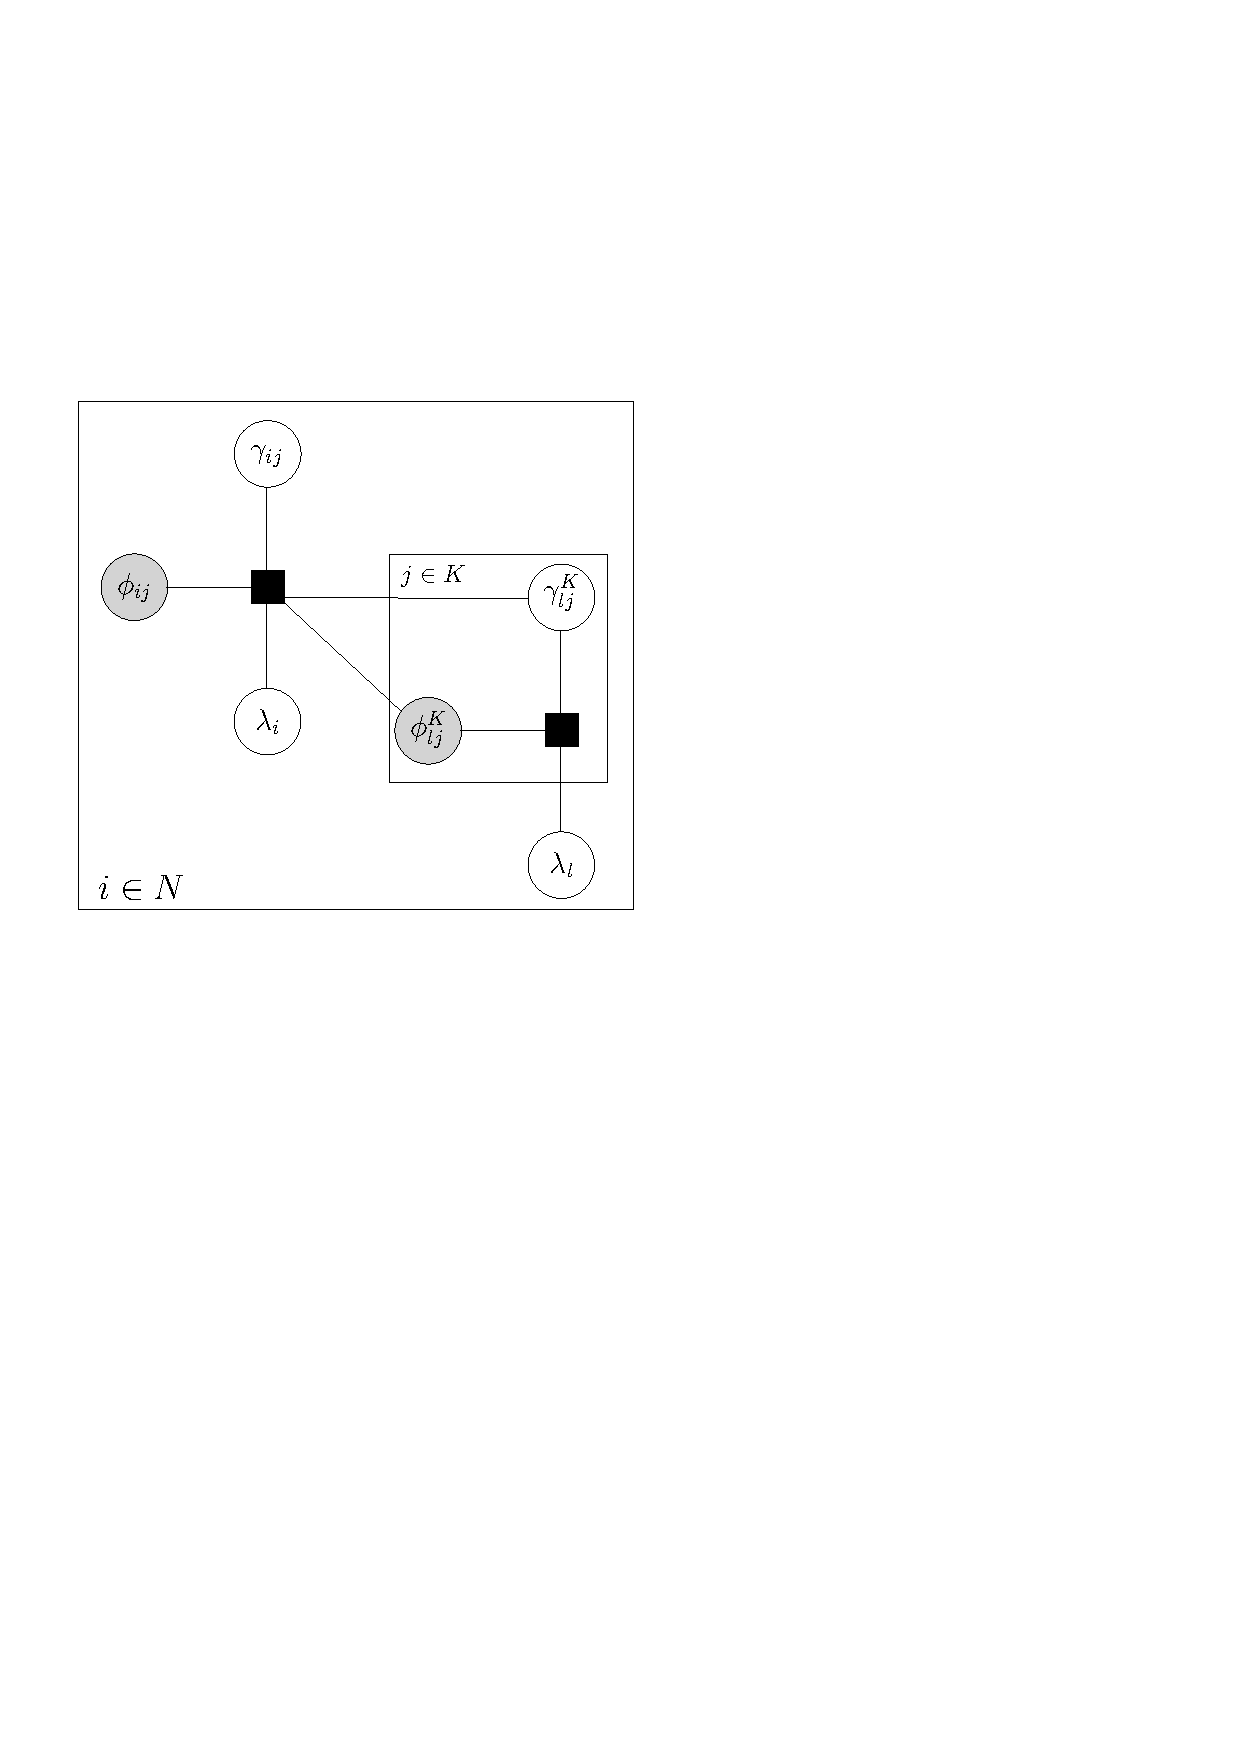
\includegraphics[width=\textwidth]{case1.pdf}
\caption{Without explicit unknown grounding variables.}
\label{fig:wo_unknown}
\end{subfigure}
~
\begin{subfigure}[t]{0.51\columnwidth}
\centering
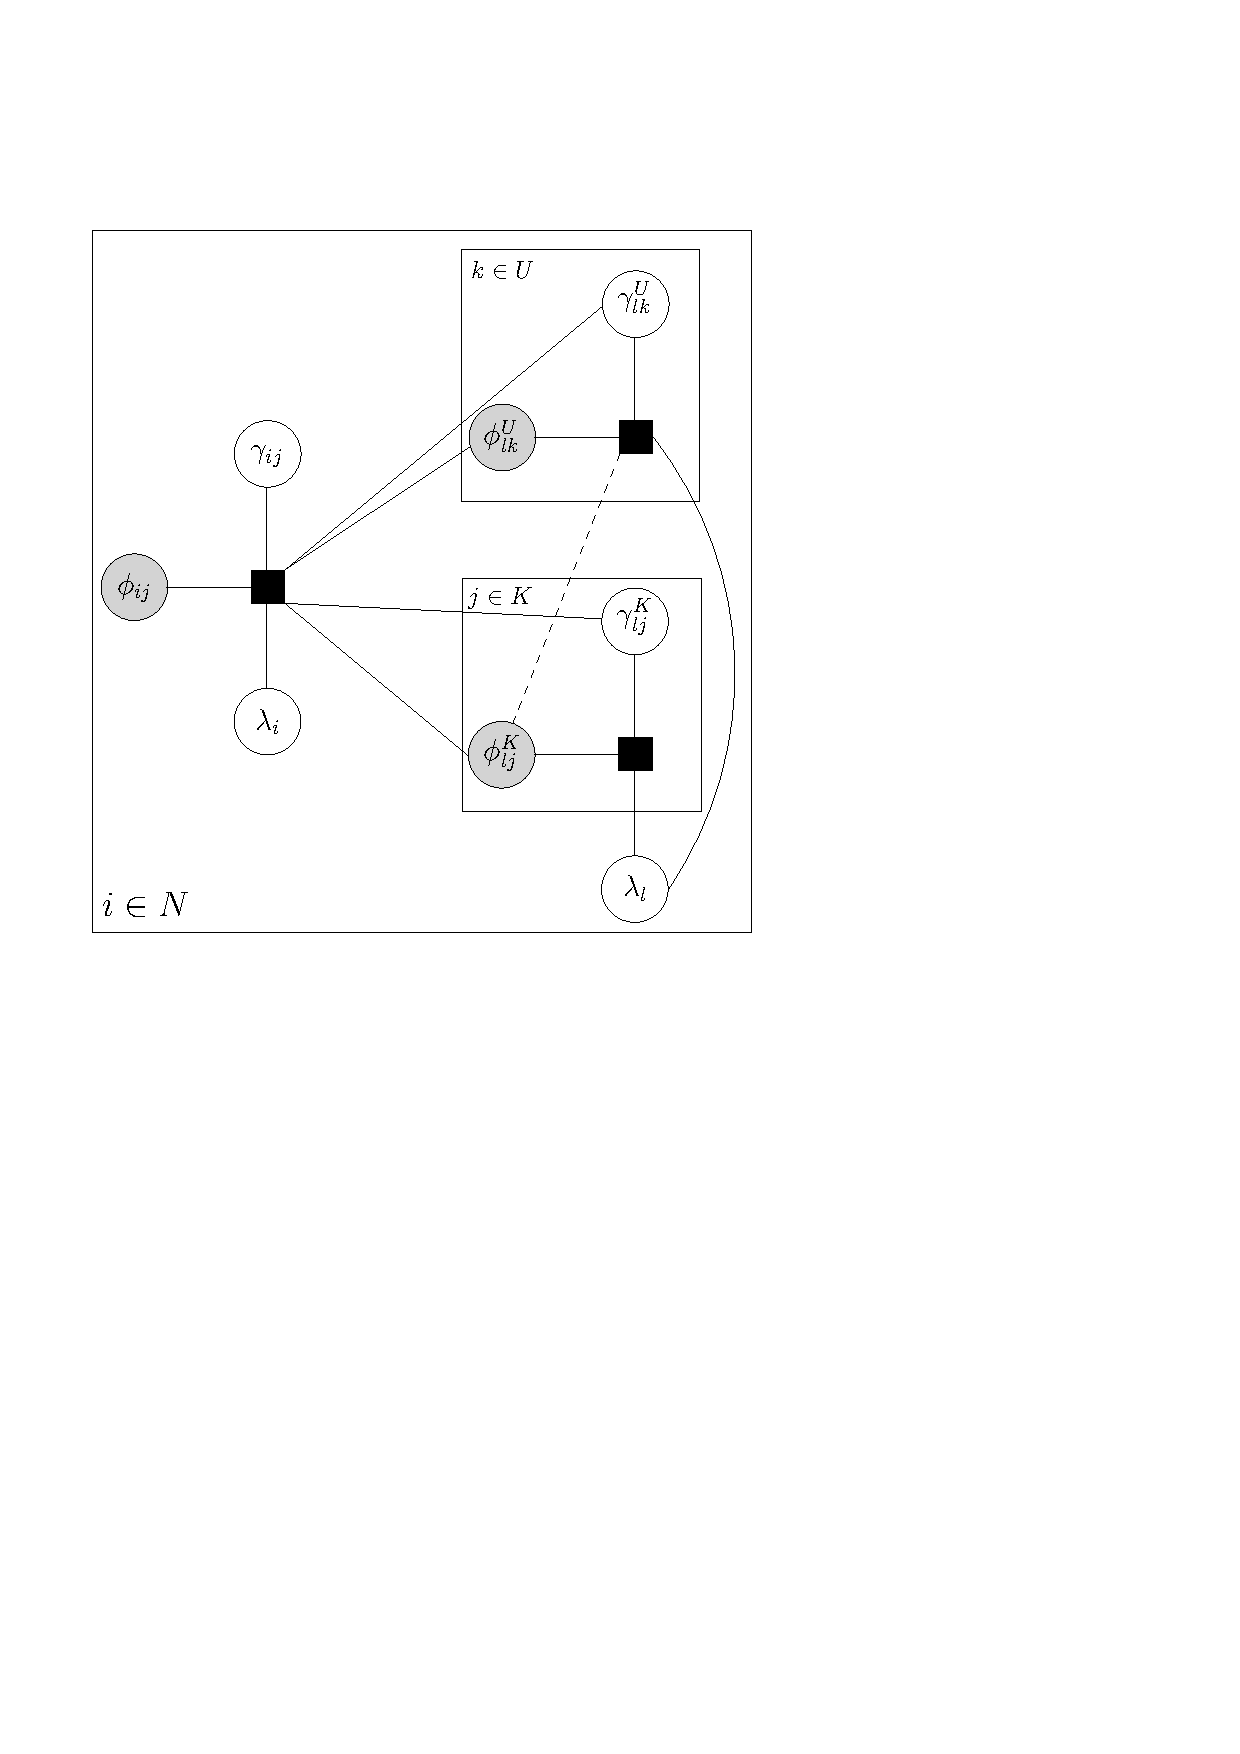
\includegraphics[width=\textwidth]{case2.pdf}
\caption{With explicit unknown grounding variables.}
\label{fig:w_unknown}
\end{subfigure}

\caption{Factor graph representations. Input instruction is parsed into $N$ phrases where $\lambda_l$ represents a child phrase of parent phrase $\lambda_i$. Superscripts $K$ and $U$ denote known and unknown variables, respectively.}
\end{figure}

\subsection{Hypothesized Groundings out of Perception}
The previous section presented that the DCG-UPUP model can explicitly represent the unknown phrases and objects. However, its performance is limited since the robot can only ground to the perceived objects. As an extension of this model, we propose the DCG-UPUP-Away, which enables to ground phrases to objects out of perception.

The main process to include hypothetical objects to the model is as follows: after populating a world model by using the sensors of the robot, a single instance of every known object type, as well as one instance of an unknown object, are added to the world model and labeled as hypothetical objects. The resulting graphical model for the DCG-UPUP-Away is illustrated in Fig.~\ref{fig:dcg-upup-away}, where the nouns may ground to 1) known and perceived objects, 2) unknown and perceived objects, 3) known and hypothetical objects, and 4) unknown and hypothetical objects. As a comparison, Fig.~\ref{fig:dcg-upup} illustrates the DCG-UPUP model, where the nouns can be grounded to only known perceived and unknown perceived objects. Moreover, Fig.~\ref{fig:dcg} presents the DCG model where the nouns can be grounded to only known perceived objects.

\begin{figure*}
\centering
\begin{subfigure}[t]{0.235\textwidth}
\centering
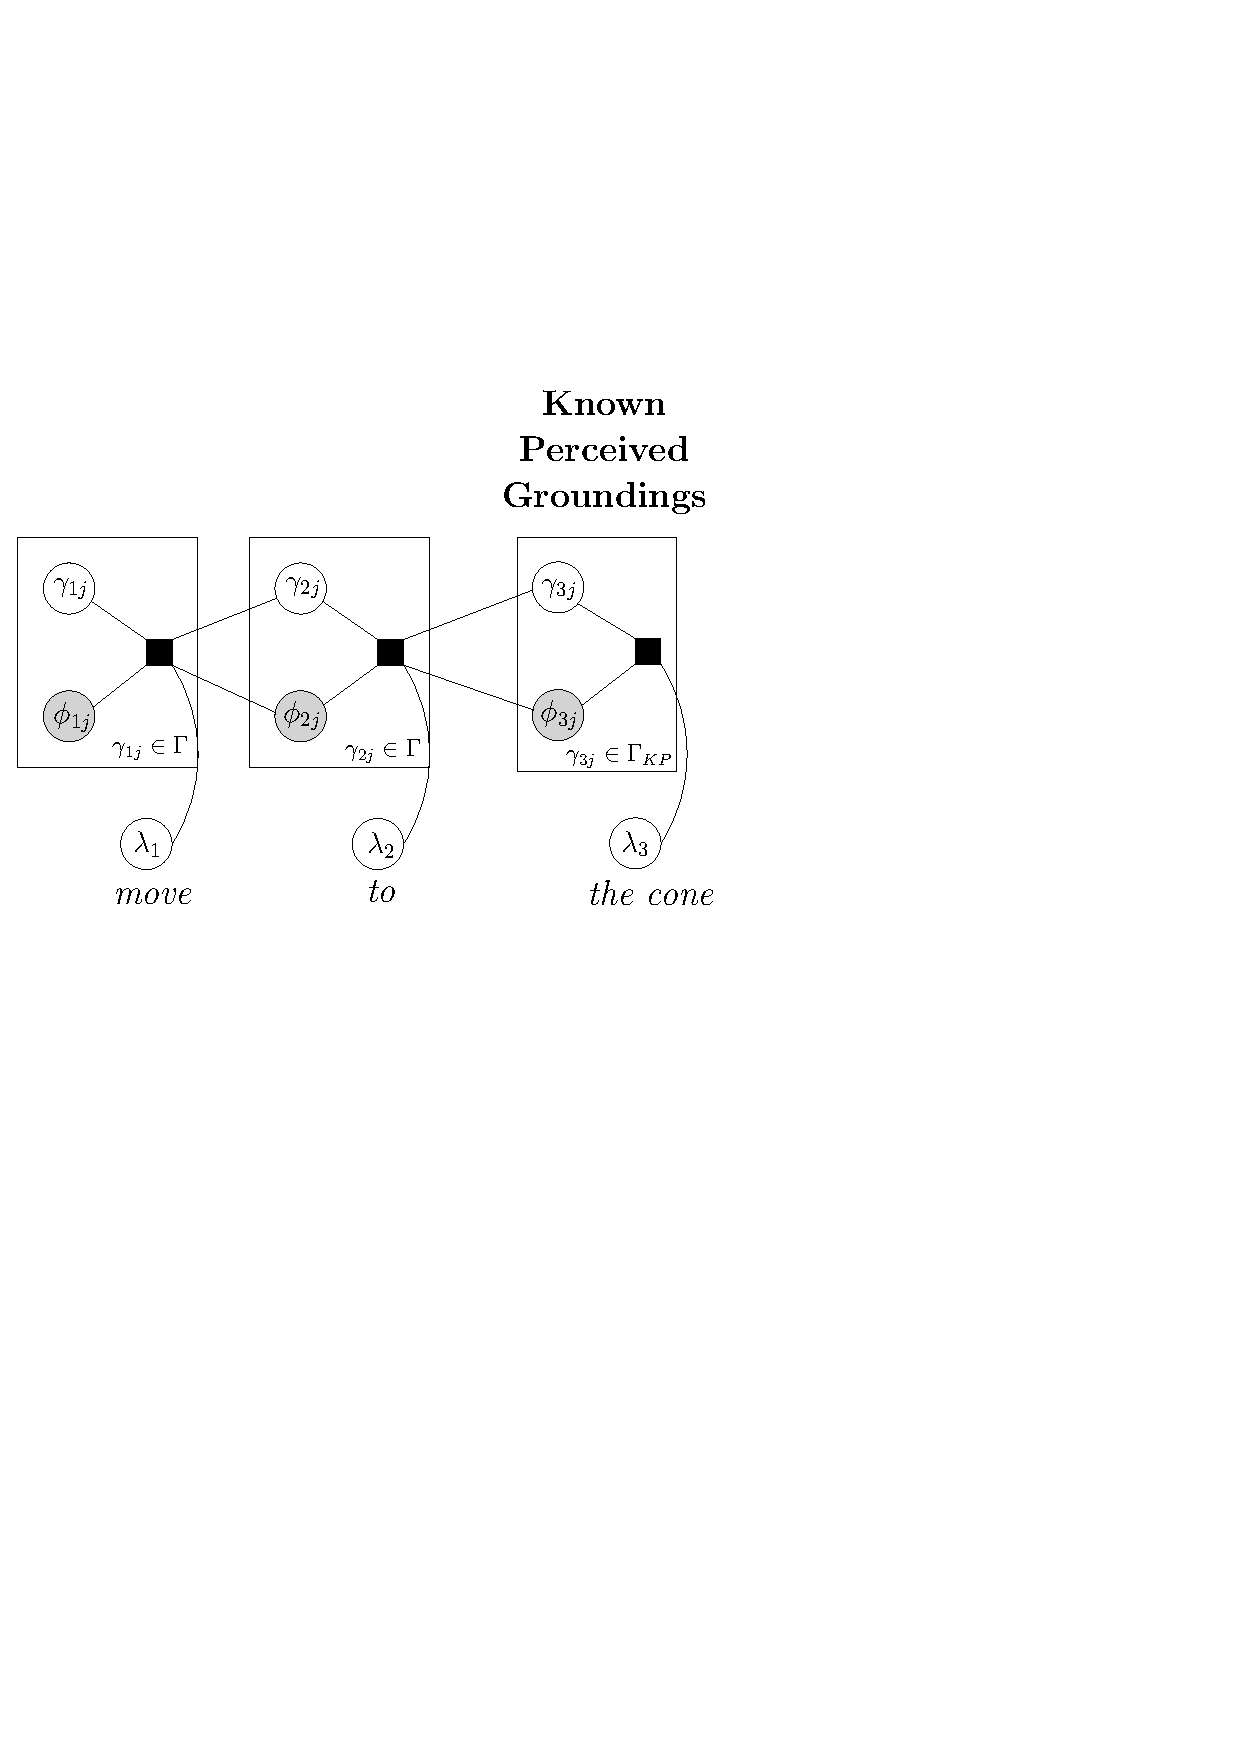
\includegraphics[width=\textwidth]{dcg.pdf}
\caption{The DCG model}
\label{fig:dcg}
\end{subfigure}
~
\begin{subfigure}[t]{0.31\textwidth}
\centering
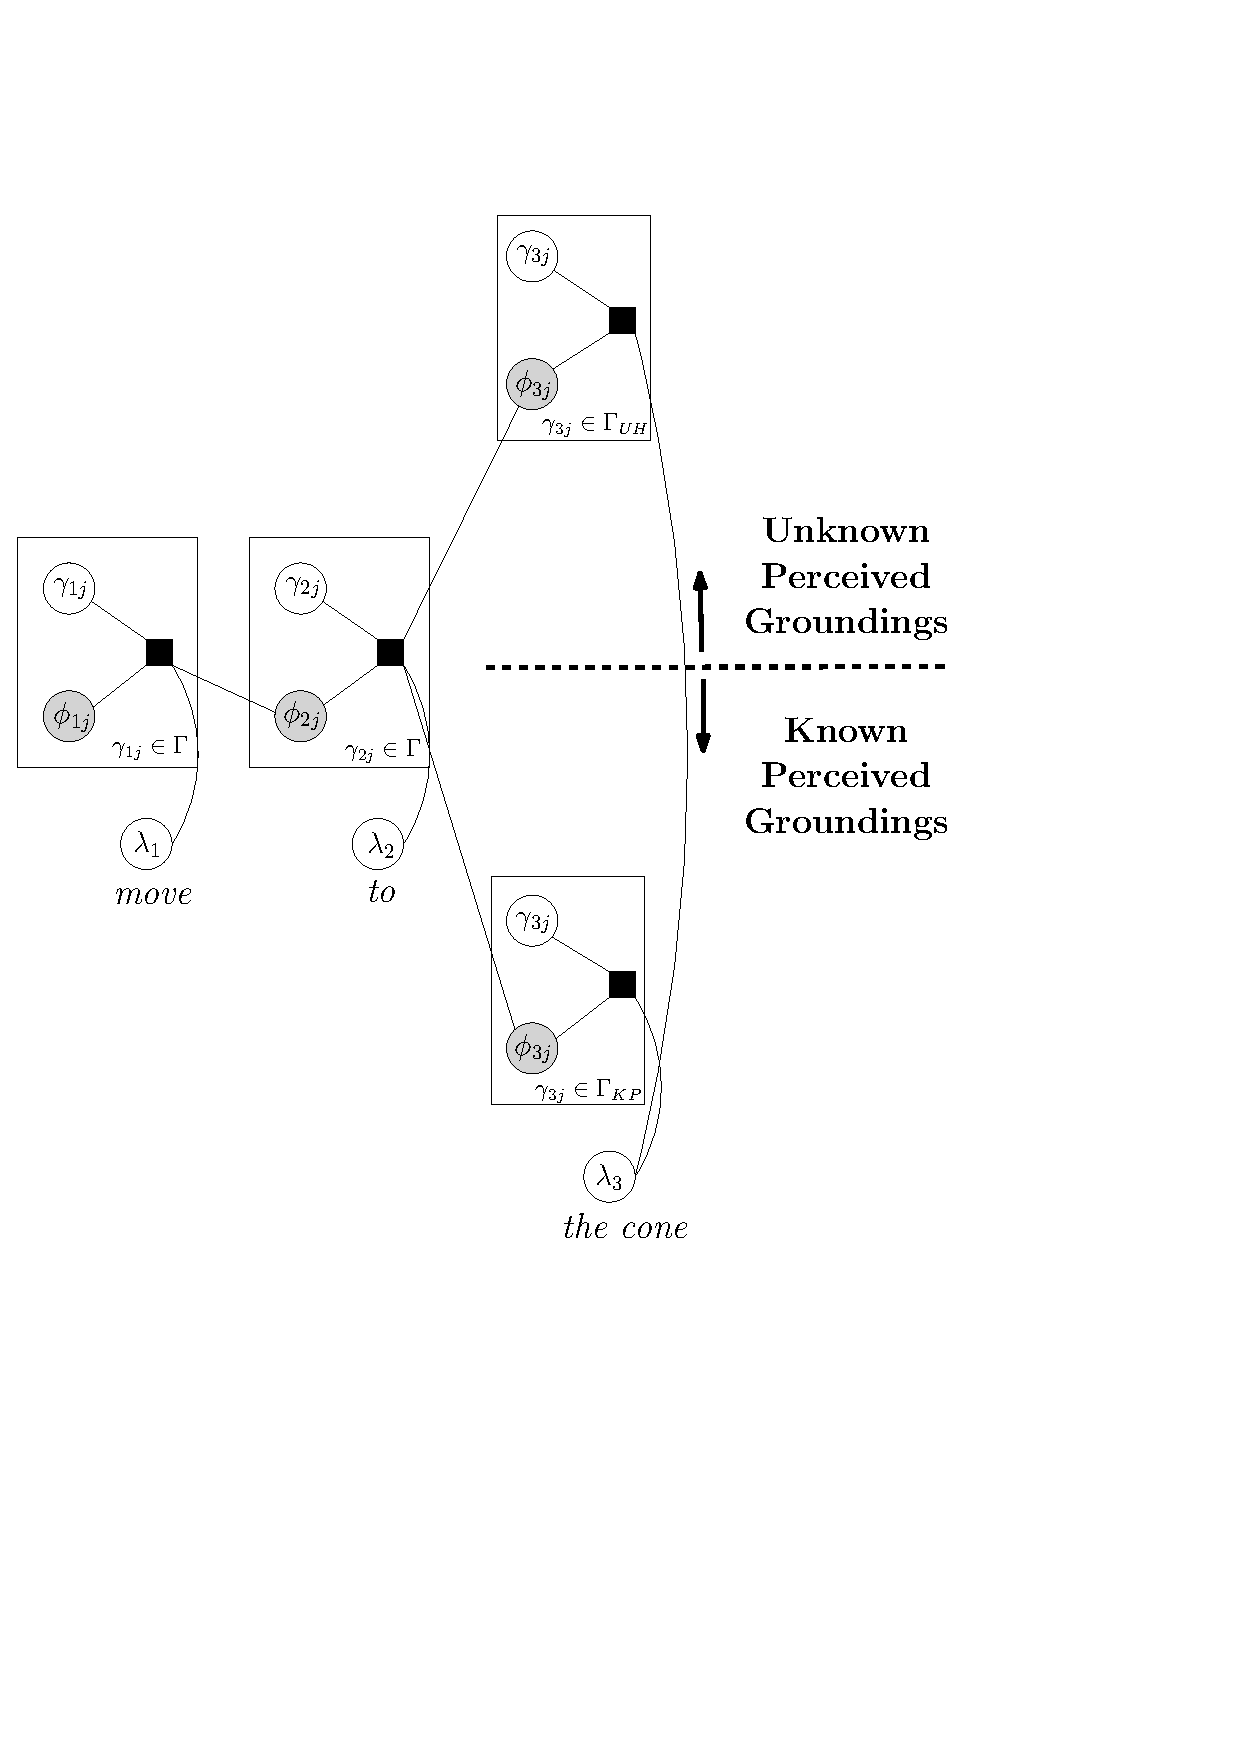
\includegraphics[width=\textwidth]{dcg_upup.pdf}
\caption{The DCG-UPUP model}
\label{fig:dcg-upup}
\end{subfigure}
~
\begin{subfigure}[t]{0.4\textwidth}
\centering
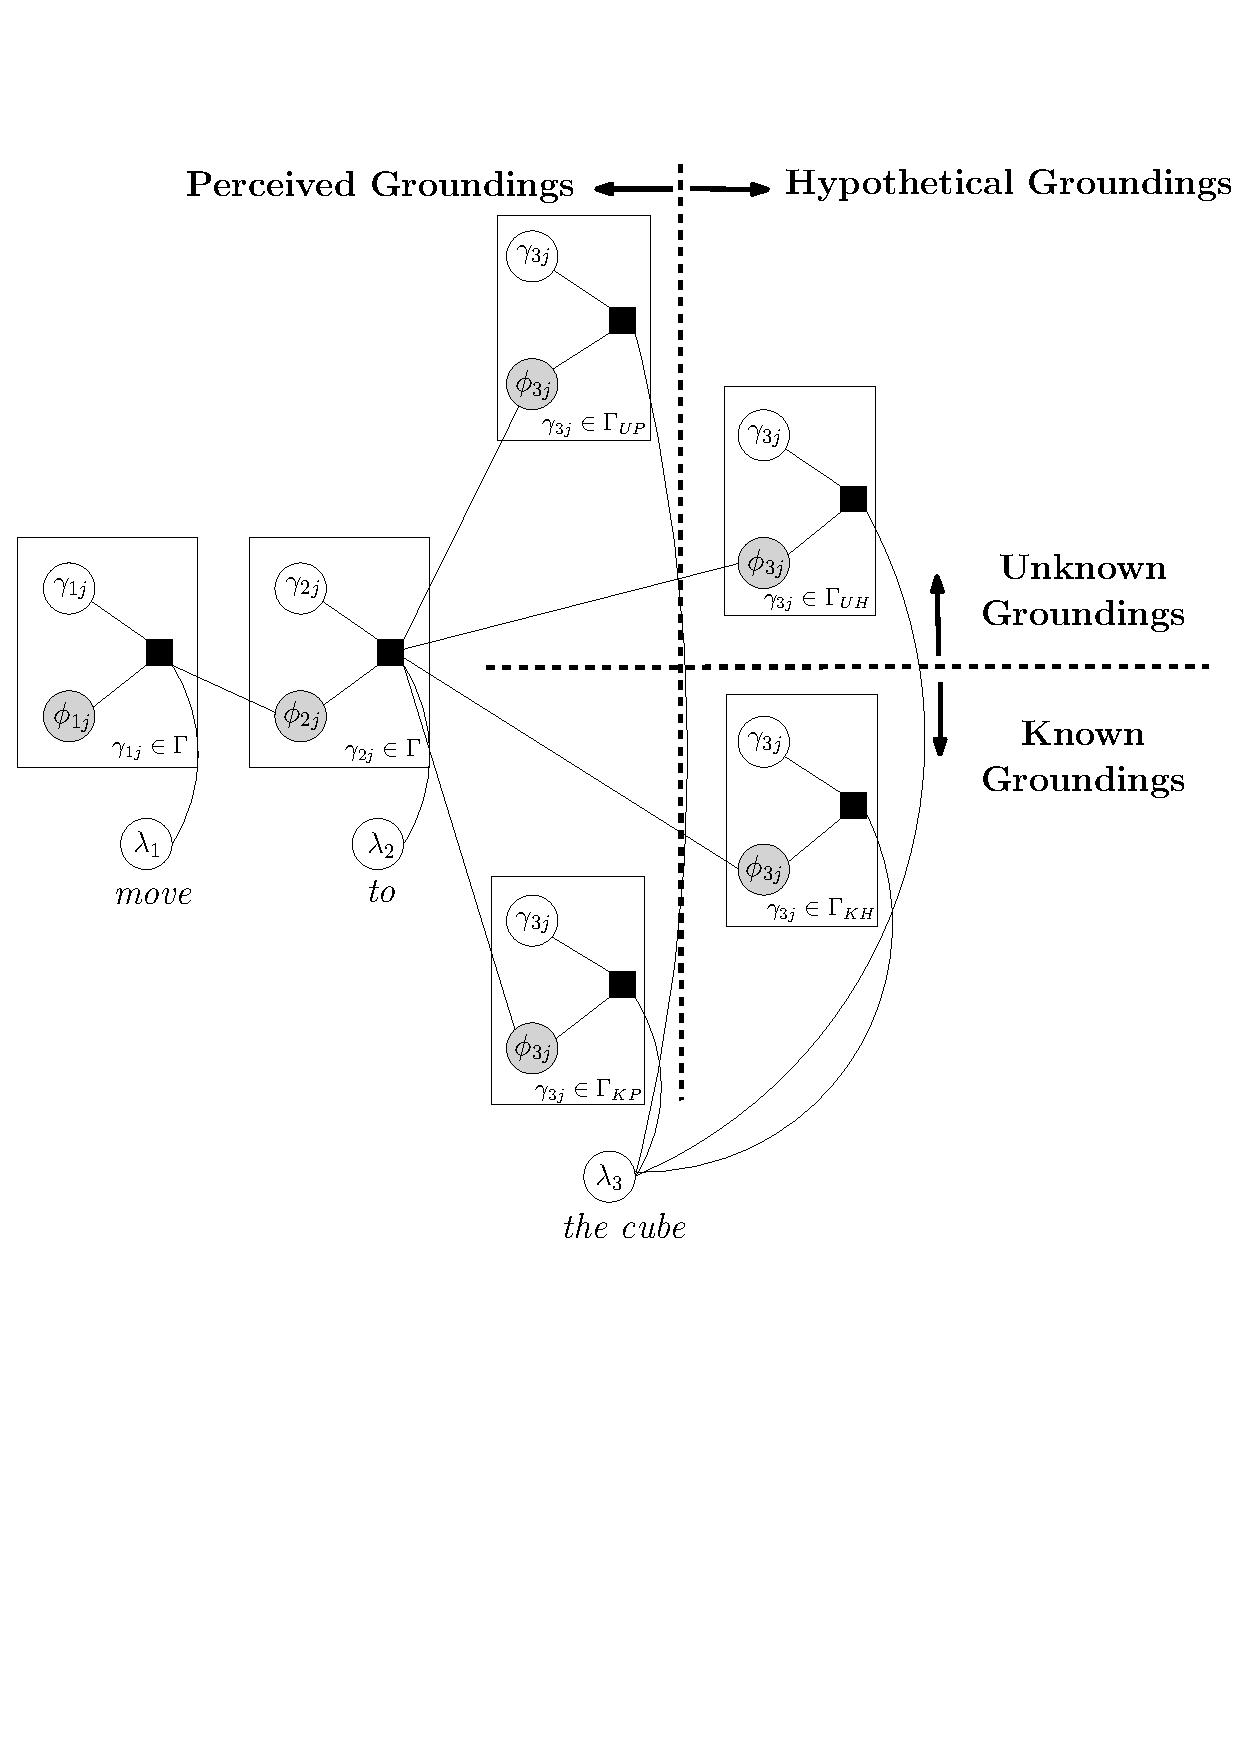
\includegraphics[width=\textwidth]{dcg_upup_away.pdf}
\caption{The DCG-UPUP-Away model}
\label{fig:dcg-upup-away}
\end{subfigure}
\caption{The graphical models constructed for the command ``\emph{move to the cone}".}
\end{figure*}

Similar to \eqref{eq:dcg_upup_llm1}, the factored objective function for the DCG-UPUP-Away model can be written by extending the world model to known perceived, unknown perceived, known hypothetical, and unknown hypothetical objects  (i.e., $\Upsilon_{KP} \cup \Upsilon_{UP} \cup \Upsilon_{KH} \cup \Upsilon_{UH}$) as follows:
\begin{equation}
\boldsymbol{\phi}^* = \argmax_{\phi_{ij} \in \boldsymbol{\phi}} \prod_{i}^{|\boldsymbol\lambda|} \prod_j^{|\Phi_i|} \Psi(\phi_{ij},\gamma_{ij},\lambda_i,\Gamma_{c_{ij}},\Upsilon_{KP} \cup \Upsilon_{UP} \cup \Upsilon_{KH} \cup \Upsilon_{UH}),
\label{eq:dcg_upup_away_llm1}
\end{equation}
where each feature function is an LLM model as:
\begin{equation}
\Psi(\phi_{ij},\gamma_{ij},\lambda_i,\Gamma_{c_{ij}},\Upsilon_{KP} \cup \Upsilon_{UP} \cup \Upsilon_{KH} \cup \Upsilon_{UH}) = \frac{A_{UH}}{B_{UH}}
\end{equation}
where
\begin{equation}
A_{UH}=\exp \Big( \sum_{f \in F_{\text{DCG}} \cup F_{U} \cup F_{H}} \mu_f f(\phi_{ij},\gamma_{ij},\lambda_i,\Gamma_{c_{ij}},\Upsilon_{KP} \cup \Upsilon_{UP} \cup \Upsilon_{KH} \cup \Upsilon_{UH}) \Big) \nonumber
%\quad \quad \quad \quad \quad \quad + \sum_{f' \in F_{U}} \mu_{f'} f'(\phi_{ij},\gamma_{ij},\lambda_i,\Gamma_{c_{ij}},\Upsilon_{KP} \cup \Upsilon_{UP} \cup \Upsilon_{KH} \cup \Upsilon_{UH}) \nonumber \\
%\quad \quad \quad \quad \quad \quad + \sum_{f^{\prime\prime} \in F_{H}} \mu_{f^{\prime\prime}} f^{\prime\prime}(\phi_{ij},\gamma_{ij},\lambda_i,\Gamma_{c_{ij}},\Upsilon_{KP} \cup \Upsilon_{UP} \cup \Upsilon_{KH} \cup \Upsilon_{UH}) \Big), \nonumber
\end{equation}

\begin{equation}
B_{UH}=\sum_{\phi_{ij} \in \{0,1\}}\exp \Big( \sum_{f \in F_{\text{DCG}} \cup F_{U} \cup F_{H}} \mu_f f(\phi_{ij},\gamma_{ij},\lambda_i,\Gamma_{c_{ij}},\Upsilon_{KP} \cup \Upsilon_{UP} \cup \Upsilon_{KH} \cup \Upsilon_{UH}) \Big) \nonumber
%\quad \quad \quad \quad \quad \quad \quad \quad + \sum_{f' \in F_{U}} \mu_{f'} f'(\phi_{ij},\gamma_{ij},\lambda_i,\Gamma_{c_{ij}},\Upsilon_{KP} \cup \Upsilon_{UP} \cup \Upsilon_{KH} \cup \Upsilon_{UH}) \nonumber \\
%\; \quad \quad \quad \quad \quad \quad \quad \quad + \sum_{f^{\prime\prime} \in F_{H}} \mu_{f^{\prime\prime}} f^{\prime\prime}(\phi_{ij},\gamma_{ij},\lambda_i,\Gamma_{c_{ij}},\Upsilon_{KP} \cup \Upsilon_{UP} \cup \Upsilon_{KH} \cup \Upsilon_{UH}) \Big), \nonumber
\end{equation}
and $F_H$ is the set of hand-coded binary features to detect if an object is hypothetical. 




\section{Implementation}
\label{sec:implementation}
\subsection{Incremental Unsupervised Learning}
While the DCG-UPUP model can reason about unknown phrases and objects, it can also learn new symbols permanently. This is mainly achieved by the following unsupervised learning procedure: whenever an unknown phrase is grounded to an unknown object, a new type is created based on the new phrase. Then, a new training example, in which the phrase grounds to the new
type, is generated. Accordingly, the LLM models are retrained with the expanded set of training examples. Consequently, when the newly generated objects (or phrases) are encountered again, they become known symbols. Hence, the DCG-UPUP model can learn to associate a new phrase with a new type.

%Here I say how we use the unknown symbol to incrementally learn more symbols.
%There's no need for extra equations, but I could include something to show how domains are expanded.
%I think that's taken care of in the pseudocode, though.

\subsection{Adjective-Attribute Heuristics}
\label{sec:color}
One way to improve the grounding performance of the DCG-UPUP-Away model is to allow the association between the natural language adjectives and the object properties. For example, if there exist two cube type objects in the world, one way to distinguish them from each other is to consider their properties such as color or size. In this section, we present how to include color information into the solution of grounding problem over the DCG-UPUP-Away. To this end, two additional features are introduced: the feature $f_{word}$ detects whether the language command contains a color adjective, and the feature $f_{color}$ checks the color property of an object.     

Note that the factored objective function in this case has exactly the same form as in \eqref{eq:dcg_upup_away_llm1} where each feature function $\Psi(.)$ is defined as follows:
\begin{equation}
\Psi(\phi_{ij},\gamma_{ij},\lambda_i,\Gamma_{c_{ij}},\Upsilon_{KP} \cup \Upsilon_{UP} \cup \Upsilon_{KH} \cup \Upsilon_{UH}) = \frac{A_{UHC}}{B_{UHC}}
\label{eq:color_llm2}
\end{equation}
where
\begin{equation}
A_{UHC}=\exp \Big( \sum_{f \in F_{\text{DCG}}} \mu_f f(\phi_{ij},\gamma_{ij},\lambda_i,\Gamma_{c_{ij}},\Upsilon_{KP} \cup \Upsilon_{UP} \cup \Upsilon_{KH} \cup \Upsilon_{UH}) \nonumber \\
\quad \quad \quad \quad \quad \quad + \sum_{f' \in F_{U}} \mu_{f'} f'(\phi_{ij},\gamma_{ij},\lambda_i,\Gamma_{c_{ij}},\Upsilon_{KP} \cup \Upsilon_{UP} \cup \Upsilon_{KH} \cup \Upsilon_{UH}) \nonumber \\
\quad \quad \quad \quad \quad \quad + \sum_{f^{\prime\prime} \in F_{H}} \mu_{f^{\prime\prime}} f^{\prime\prime}(\phi_{ij},\gamma_{ij},\lambda_i,\Gamma_{c_{ij}},\Upsilon_{KP} \cup \Upsilon_{UP} \cup \Upsilon_{KH} \cup \Upsilon_{UH}) \nonumber \\
\quad \quad \quad \quad \quad \quad + \sum_{f^{\prime\prime\prime} \in F_{C}} \mu_{f^{\prime\prime\prime}} f^{\prime\prime\prime}(\phi_{ij},\gamma_{ij},\lambda_i,\Gamma_{c_{ij}},\Upsilon_{KP} \cup \Upsilon_{UP} \cup \Upsilon_{KH} \cup \Upsilon_{UH}) \Big), \nonumber
\end{equation}

\begin{equation}
B_{UHC}=\sum_{\phi_{ij} \in \{0,1\}}\exp \Big( \sum_{f \in F_{\text{DCG}}} \mu_f f(\phi_{ij},\gamma_{ij},\lambda_i,\Gamma_{c_{ij}},\Upsilon_{KP} \cup \Upsilon_{UP} \cup \Upsilon_{KH} \cup \Upsilon_{UH}) \nonumber \\
\quad \quad \quad \quad \quad \quad \quad \quad + \sum_{f' \in F_{U}} \mu_{f'} f'(\phi_{ij},\gamma_{ij},\lambda_i,\Gamma_{c_{ij}},\Upsilon_{KP} \cup \Upsilon_{UP} \cup \Upsilon_{KH} \cup \Upsilon_{UH}) \nonumber \\
\quad \quad \quad \quad \quad \quad \quad \quad + \sum_{f^{\prime\prime} \in F_{H}} \mu_{f^{\prime\prime}} f^{\prime\prime}(\phi_{ij},\gamma_{ij},\lambda_i,\Gamma_{c_{ij}},\Upsilon_{KP} \cup \Upsilon_{UP} \cup \Upsilon_{KH} \cup \Upsilon_{UH})\nonumber \\
\; \quad \quad \quad \quad \quad \quad \quad \quad + \sum_{f^{\prime\prime\prime} \in F_{C}} \mu_{f^{\prime\prime\prime}} f^{\prime\prime\prime}(\phi_{ij},\gamma_{ij},\lambda_i,\Gamma_{c_{ij}},\Upsilon_{KP} \cup \Upsilon_{UP} \cup \Upsilon_{KH} \cup \Upsilon_{UH}) \Big), \nonumber
\end{equation}
and $F_C$ is the set of hand-coded binary features for detecting color phrases or properties (i.e., $F_C = f_{color} \cup f_{word}$).


\begin{algorithm}[b!]\footnotesize
\caption{Grounding/Learning over DCG-UPUP-Away}\label{alg:dcg_upup_away}
\begin{algorithmic}[1]
\Procedure{DCG-UPUP-Away}{}
\State $M \gets \text{new DCG-UPUP-Away}$
\State $M.\Gamma \gets \text{init\_groundings}$
\State $M.F \gets \text{init\_features}$
\State $T \gets \text{init\_training}$
\State $M.\text{train}(M.\Gamma, M.F, T)$
\While {true}
\State $\Upsilon \gets \text{perceive\_objects}(\text{camera},M.\Gamma)$
\State $\Upsilon \gets \Upsilon + \text{hypothesize\_objects}(M.\Gamma)$
\State $\boldsymbol{\lambda} \gets \text{get\_nl\_command}()$
\State $[\boldsymbol{\phi}^*,\boldsymbol{\gamma}^*] \gets M.\text{ground}(\boldsymbol{\lambda},\Upsilon)$
\If {$\boldsymbol{\gamma}^*.\text{is\_hypothesized}()$}
\State $\text{explore\_surroundings()}$
\Else
\State $\text{drive\_to}(\boldsymbol{\gamma}^*)$
\EndIf
\State $T_u \gets \text{gen\_unsupervised\_training}(\boldsymbol{\lambda},\boldsymbol{\gamma}^*,\Upsilon)$
\If {$\text{is\_unknown}(\boldsymbol{\lambda}) \& !\boldsymbol{\gamma}^*.\text{is\_hypothesized}()$}
\State $\gamma' \gets \text{new\_grounding}(\boldsymbol{\lambda},\boldsymbol{\gamma}^*,\Upsilon)$
\State $M.\Gamma \gets M.\Gamma + \gamma'$
\State $M.F \gets M.F + f_{\text{word}}(\boldsymbol{\lambda}[\text{noun}])$
\State $M.F \gets M.F + f_{\text{color}}(\boldsymbol{\gamma}^*[\text{color}])$
\State $M.F \gets M.F + f_{\text{obj}}(\boldsymbol{\gamma}^*[\text{obj}])$
\State $T_u \gets \text{replace\_unknown}(T_u,\gamma')$
\EndIf
\State $T \gets T + T_u$
\State $M.\text{train}(M.\Gamma, M.F, T)$
\EndWhile
\EndProcedure
\end{algorithmic}
\end{algorithm}
\subsection{Overview of the Pseudo-code}
The pseudo-code for grounding and learning new symbols over the DCG-UPUP-Away model is presented in Alg.~\ref{alg:dcg_upup_away}. First, the graphical model $M$ is initialized and trained with the initial set of training data (lines 1-6). Grounding to unknown symbols and/or hypothetical objects are tackled between the lines 7-24. In particular, the world model is updated with the perceived objects (line~8) and then hypothetical objects are added (line~9). The natural language command is entered as an input (line~10). Using the model $M$ with the language command $\boldsymbol\lambda$ and the most recent world model $\Upsilon$, the grounding problem is solved (line~11). If the obtained grounding is hypothetical, then the robot initiates the exploration (line~13); otherwise the robot moves towards the grounded perceived object (line~15). Note that the exploration in this research is considered as the robot rotating in its current location. At the end of solving the grounding problem, a new training file is generated based on the given command $\boldsymbol\lambda$, the resulting grounding $\boldsymbol\gamma^*$, and the current world model $\Upsilon$ (line~16). If there exists an unknown phrase in the given command and the resulting grounding is not hypothetical, then a new object type (or grounding variable) is generated (line~18) and the set of grounding variables as well as the feature sets are updated (lines~19-22). Finally, the newly generated object type $\gamma^\prime$ replaces the unknown object type in training file $T_u$ (line~23), and the model $M$ is retrained with the new set of training data. Consequently, the initially unknown object becomes a known object in the new model $M$ in the further iterations. 



%\begin{equation}
%\Psi() = \exp \Big( \sum_{f \epsilon F_{\text{DCG}}} \mu_f f(\phi_{ij},\gamma_{ij},\lambda_i,\Gamma_{c_{ij}},\Upsilon_{KP} \cup \Upsilon_{UP} \cup \Upsilon_{KH} \cup \Upsilon_{UH}) +...\\
%\sum_{f' \epsilon F_{\text{Unknown}}} \mu_{f'} f'(\phi_{ij},\gamma_{ij},\lambda_i,\Gamma_{c_{ij}},\Upsilon_{KP} \cup \Upsilon_{UP} \cup \Upsilon_{KH} \cup \Upsilon_{UH}) +...\\
%\mu_{f_H} f_{H}(\phi_{ij},\gamma_{ij},\lambda_i,\Gamma_{c_{ij}},\Upsilon_{KP} \cup \Upsilon_{UP} \cup \Upsilon_{KH} \cup \Upsilon_{UH}) +...\\
%\sum_{f'' \epsilon F_{\text{Color}}} \mu_{f''} f''(\phi_{ij},\gamma_{ij},\lambda_i,\Gamma_{c_{ij}},\Upsilon_{KP} \cup \Upsilon_{UP} \cup \Upsilon_{KH} \cup \Upsilon_{UH}) \Big)
%\label{eq:color_llm2}.
%\end{equation}